Программное решение представлено на языке \textit{Go}. Причины для использования этого языка при написании вычислительных параллельных задач следующие:
\begin{enumerate}
    \item Go --- компилируемый язык со встроенной сборкой мусора. Это необычное сочетание качеств колоссально повышает скорость разработки, при этом язык проигрывает в производительности языку C всего в 1,5--2 раза.
    \item Go представляет современные средства параллелелизма \textit{go routines}. В отличие от классических потоков (threads) рутины управляются не операционной системой, а \textit{go runtime}, за счет чего значительно сокращаются накладные расходы на создание таких рутин и на коммуникацию между ними.
\end{enumerate}

Помимо основных алгоритмов были написаны сопутствующие программы для генрации начальных данных и визуализации результатов. Генерация карты высот происходит посредством последовательного сложения нескольких шумов Перлина с подобранными различными параметрами для получения похожего на земной ландшафта \cite{perlin}. Карту с различными типами почв и фазовыми ограничениями предлагается самостоятельно нарисовать пользователю в любом графическом редакторе, например, Microsoft Paint, перед запуском программы.

В случае распрараллелевания на многонодной установке, программа поставляется в виде двух docker-образов и Ku\-ber\-ne\-tes манифестов для последовательного применения для деплоя на кластер, оркестрируемый Kubernetes. На других облачных оркестраторах решение не проверялось. Написание Ku\-ber\-ne\-tes оператора для данного решения видится нецелесообразным, ввиду отсутствия у программы сложного жизненного цикла.

Визуализация сделана с помощью платформо-независимой спецификации OpenGL, что позволяет собирать все компоненты под различные операционный системы. Ниже представлены несколько примеров работы программы. Все алгоритмы выдают одинаковый результат, однако всвязи с разной асимптотической сложностью, алгоритм Беллмана--Форда имеют размер сетки на порядок меньше, чем для алгоритма Дейстры.

В примерах ниже, время перехода принято равным
\[
    d_{i,j}(\hat i, \hat j) = 100\cdot(\mathrm{height}(\hat i, \hat j) - \mathrm{height}(i, j))_{+} + 5.
\]

\begin{figure}[h]
    \centering
    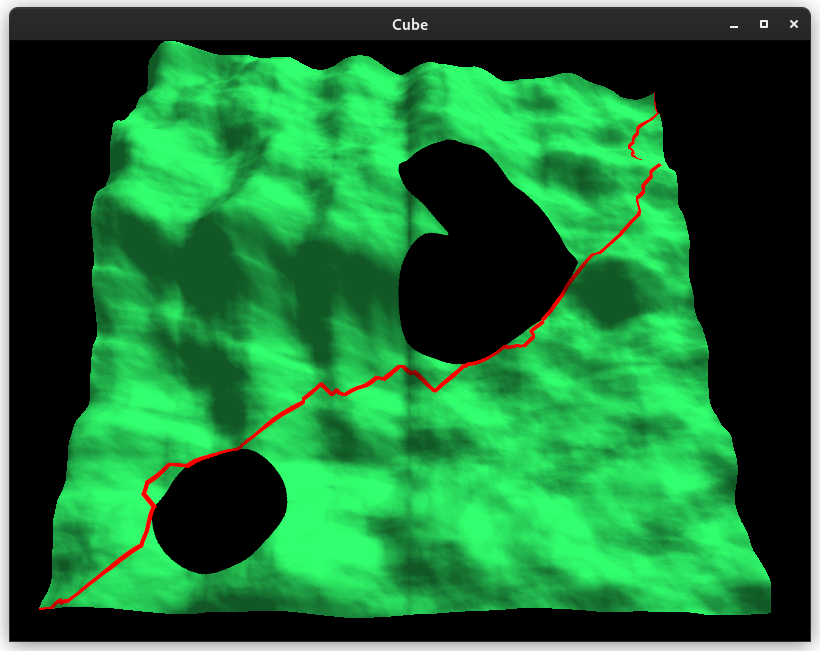
\includegraphics[scale=0.5]{content/dijkstra-top.png}
    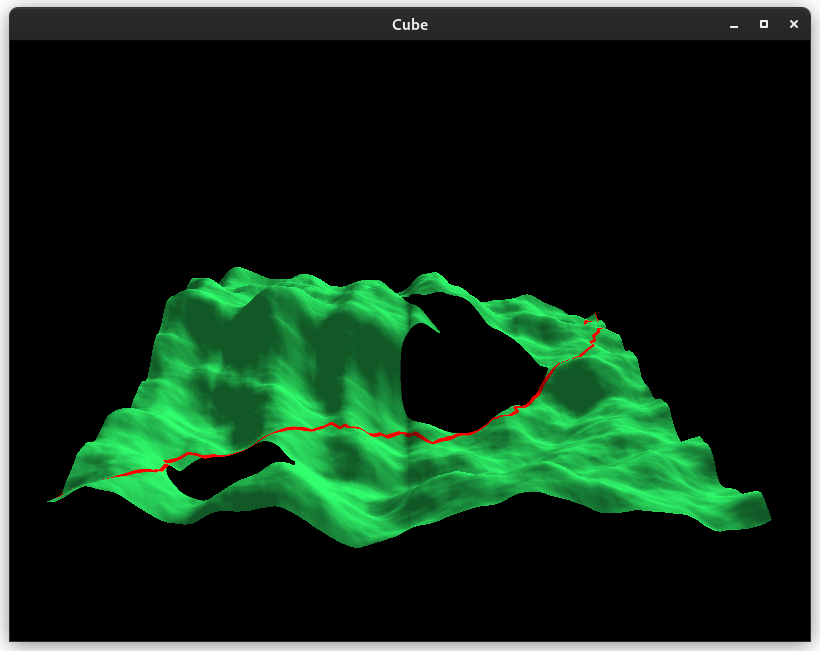
\includegraphics[scale=0.5]{content/dijkstra.png}
    \caption{Результат работы алгоритма Дейкстра на сетке 1000$\times$1000 c начальной позицией $(1, 1)$, конечной $(1000, 1000)$.}
\end{figure}

\begin{figure}[h]
    \centering
    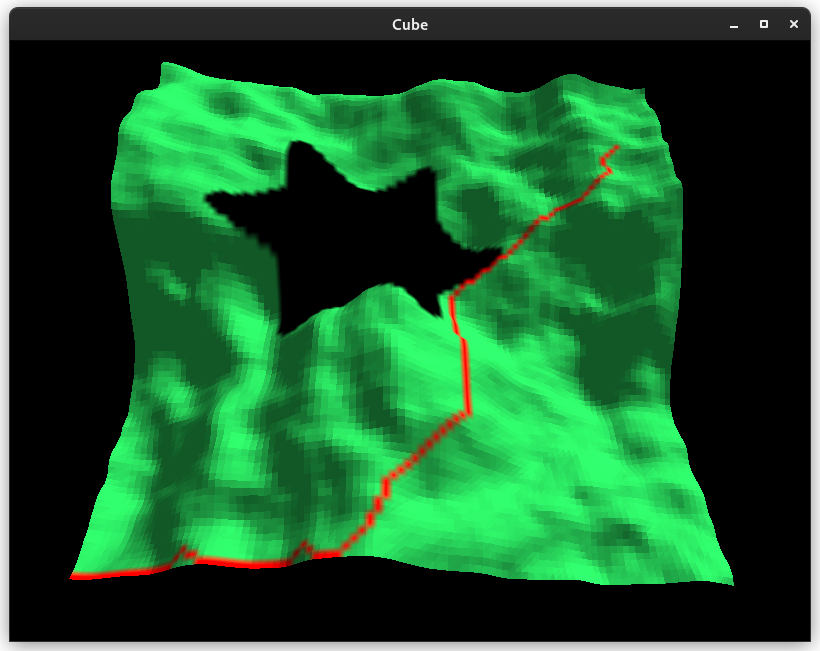
\includegraphics[scale=0.5]{content/bf-top.png}
    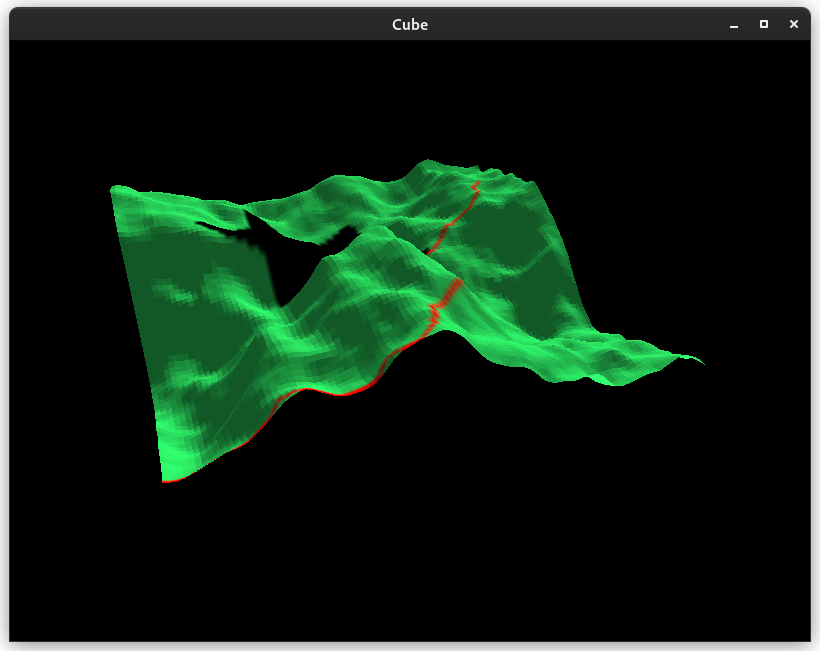
\includegraphics[scale=0.5]{content/bf.png}
    \caption{Результат работы алгоритма Беллмана--Форда на сетке 100$\times$100 c начальной позицией $(1, 1)$, конечной $(90, 90)$.}
\end{figure}
\clearpage